\chapter{Specific Requirements}

\section{External Interface Requirements}
\subsection{User Interfaces}
\subsection{Hardware Interfaces}
This section describes the logical and physical characteristics of each interface 
between the hardware and software componenents of the system.\\
Both educators and students need to have a computer to use the CKB platform.\\
\subsection{Software Interfaces}
This section describes the connections between the system and other specific software components.\\
CodeKataBattle is a web application, so it needs a web browser to be used.\\
\subsection{Communication Interfaces}
This section describes the requirements associated with any communication function required
by this system.\\
All the communications of the eMall infrastructure are made via the HTTP application layer
protocol: obviously, all the devices using the platform must be connected via WiFi or mobile
network (LTE/3G/4G/5G).\\

\section{Functional Requirements}
\subsection{Use Cases Diagrams}
\begin{figure}[H]
    \centering
    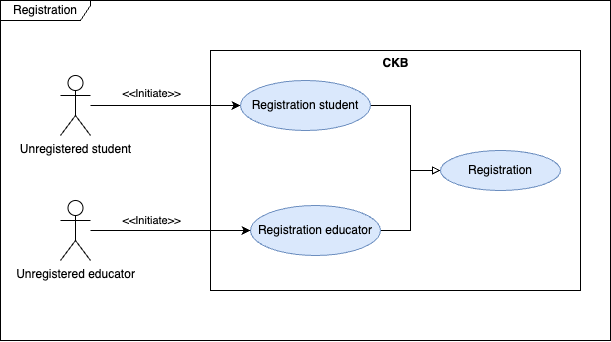
\includegraphics[width=0.8\textwidth]{images/use_cases_diagrams/Registration.png}
    \caption{Unregistered user (student or educator) use case diagram}
    \label{fig:use_case_diagram}
\end{figure}
\clearpage

\subsection{Use Cases Description}
\usecase
{1}
{Login}
{Student, Educator}
{The actor is already registered in the system.}
{
    \begin{enumerate}
        \item The actor requires the Login Page.
        \item The system shows the Login Page to the actor.
        \item The actor inserts the credentials (email and passwors) in the form.
        \item The actor submits the form and sends it to the system.
        \item The system processes the information and shows a success message redirecting the user to the homepage.
    \end{enumerate}
}
{The actor is correctly logged in and the homepage is displayed.}
{
    The provided email or password submitted is wrong.
}
{
    In case of exception the system will notify user with a human-readable message.
}
\clearpage

\usecase
{2}
{Registration} % name
{Student, Educator, Email Service, GitHub Service} % actor
{The actor browses and opens the webapp.} % entry condition
{ % event flow
    \begin{enumerate}
        \item The actor clicks the 'Sign up' button.
        \item The actor fills the sign-up form with email and password and submits the form.
        \item The system calls Email Service API to send to the actor an email containing a secret code.
        \item The Email Service sends the email to the actor.
        \item The actor submits the received verification code.
        \item The system displays a success message.
        \item The actor adds his personal information (name, surname, birth date) and submits the form.
        \item The student adds his GitHub username and submits the information.
        \item The system calls GitHub Service API to check if the username is valid.
        \item The GitHub Service sends the response to the system.
        \item The system displays a success message about the verification of GitHub username.
        \item The system processes the provided information and creates a new account.
    \end{enumerate}
}
{The actor signed up correctly.} % exit condition
{ % exceptions
    \begin{enumerate}
        \item A required registration field is missing when the form is submitted.
        \item A provided email is already registered in the system.
        \item A wrong verification code is submitted.
        \item A wrong GitHub username is submitted.
    \end{enumerate}
}
{ % notes
In case of exception the system will notify user with a human-readable message.
}

\usecase
{10}
{Evaluation} % name
{Student, Educator, GitHub Service} % actor
{The student has committed the code.} % entry condition
{ % event flow
    \begin{enumerate}
        \item The student pushes the code to GitHub.
        \item The GitHub service notify the system about the new push.
        \item The system pulls the code from GitHub service.
        \item The GitHub service provides the requested code to the system.
        \item The system makes the automatic evaluation.
        \item The system sets the calcutaed score to the code.
        \item The system notify the student about the evaluation and the score assigned to his code.
        \item The educator can get the code from the system.
        \item The system provides the code to the educator.
        \item The educator can manually evaluate the code at the end of the battle and set a score.
        \item The system updates the score.
    \end{enumerate}
}
{The system sends an email to the students.} % exit condition
{ % exceptions
 None. 
}
{ % notes
}
\clearpage

\usecase
{14}
{Profile visualization} % name
{Student, Educator} % actor
{The actor is logged-in in the system.} % entry condition
{ % event flow
    \begin{enumerate}
        \item The actor searches a student profile.
        \item The system returns the selected student profile.
    \end{enumerate}
}
{The actor visualizes the personal information of the student.} % exit condition
{ % exceptions
 The selected profile does not exist. 
}
{ % notes
In case of exception the system will notify user with a human-readable message.
}

\subsection{Sequence Diagrams}
\begin{figure}[H]
    \centering
    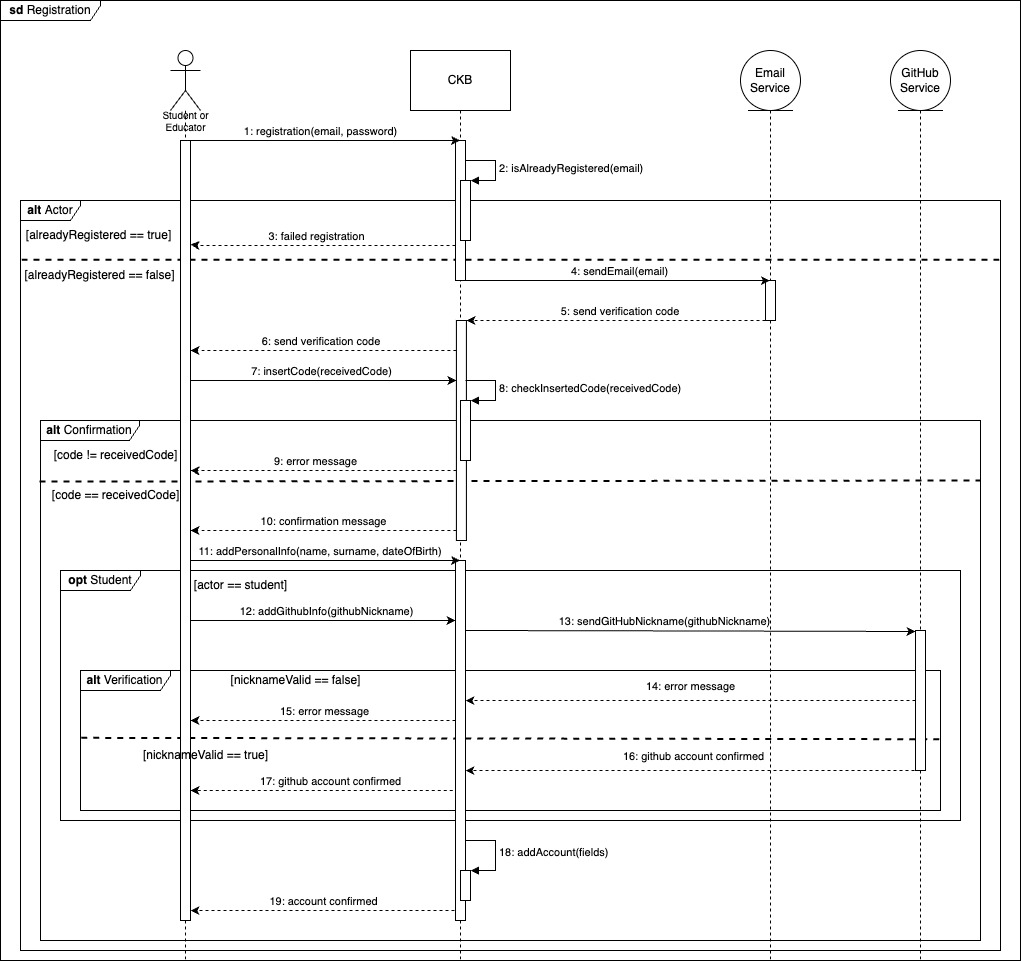
\includegraphics[width=0.95\textwidth]{images/seq_diagrams/Registration.jpg}
    \caption{Registration sequence diagram}
    \label{fig:sequence_diagram}
\end{figure}
\clearpage

\begin{figure}[H]
    \centering
    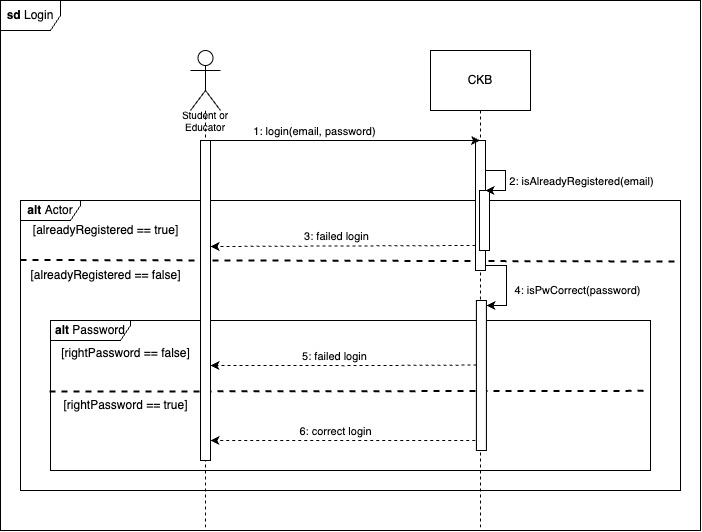
\includegraphics[width=0.95\textwidth]{images/seq_diagrams/Login.jpg}
    \caption{Login sequence diagram}
    \label{fig:sequence_diagram}
\end{figure}
\clearpage

\begin{figure}[H]
    \centering
    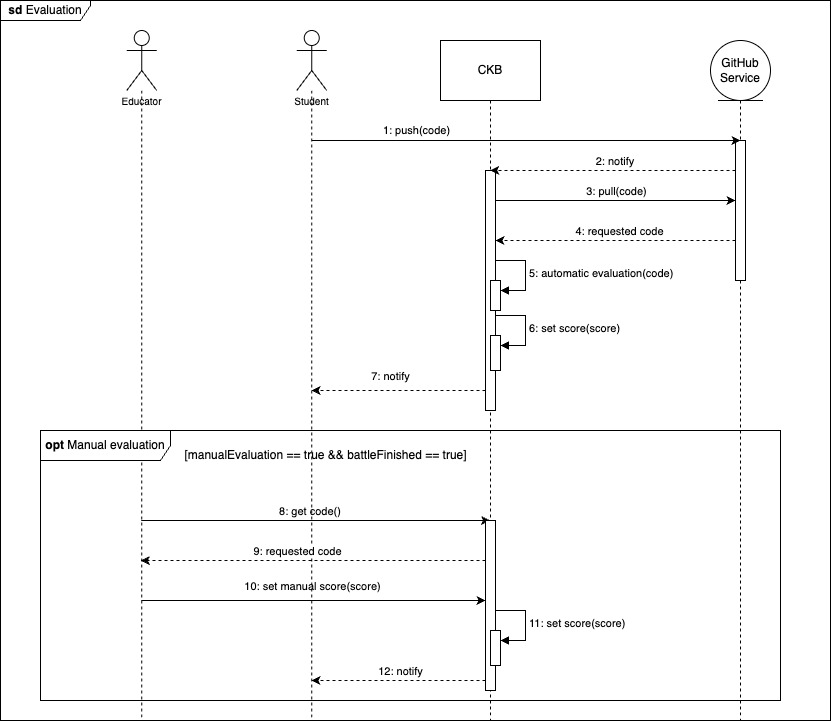
\includegraphics[width=0.95\textwidth]{images/seq_diagrams/Evaluation.jpg}
    \caption{Evaluation sequence diagram}
    \label{fig:sequence_diagram}
\end{figure}
\clearpage

\begin{figure}[H]
    \centering
    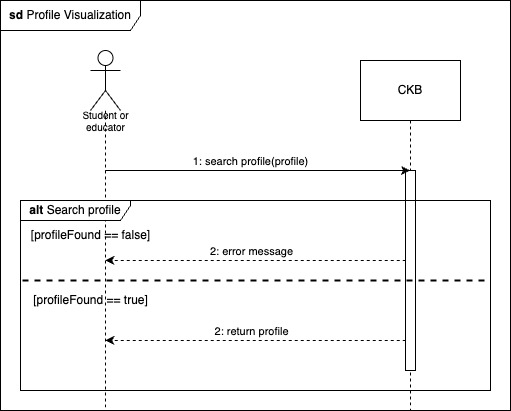
\includegraphics[width=0.9\textwidth]{images/seq_diagrams/ProfileVis.jpg}
    \caption{Profile visualization sequence diagram}
    \label{fig:sequence_diagram}
\end{figure}
\clearpage

\section{Design Constraints}
\subsection{Standards compliance}
\subsection{Hardware limitations}
\subsection{Any other constraint}

\section{Software System Atttributes}
\subsection{Reliability}
\subsection{Availability}
\subsection{Security}
\subsection{Maintainability}
\subsection{Portability}